\documentclass{ximera}

\begin{document}
	\author{Stitz-Zeager}
	\xmtitle{The Dot Product}{}


\mfpicnumber{1}

\opengraphsfile{TheDotProduct}

\setcounter{footnote}{0}

\label{TheDotProduct}

In Section \ref{Vectors}, we learned how add and subtract vectors and how to multiply vectors by scalars.  In this section, we define a product of vectors.  We begin with the following definition.

 
%% \colorbox{ResultColor}{\bbm
\begin{definition} \label{dotproductdefn}    Given vectors  $\overrightarrow{v} = \left<v_1,v_2\right>$ and $\overrightarrow{w} = \left<w_1,w_2\right>$,  the \textbf{dot product}\index{vector ! dot product ! definition of}\index{vector ! scalar product ! definition of}\index{dot product ! definition of} of $\overrightarrow{v}$ and $\overrightarrow{w}$ is given by

\[ \overrightarrow{v} \cdot \overrightarrow{w} = \left<v_1,v_2\right> \cdot \left<w_1,w_2\right> = v_1w_1 + v_2w_2 \]


 


\end{definition}
%% \ebm}

 

For example, if $\overrightarrow{v} = \left<3,4\right>$ and $\overrightarrow{w} = \left<1,-2\right>$,then $\overrightarrow{v} \cdot \overrightarrow{w} = \left<3,4\right> \cdot \left<1,-2\right> =  (3)(1) + (4)(-2) = -5$. 

 

Note that the dot product takes two \textit{vectors} and produces a \textit{scalar}.  For that reason, the quantity $\overrightarrow{v} \cdot \overrightarrow{w}$ is often called the \textbf{scalar product} of $\overrightarrow{v}$ and $\overrightarrow{w}$.  The dot product enjoys the following properties.

 

%% \colorbox{ResultColor}{\bbm

\begin{theorem} \label{dotprodprops} \textbf{Properties of the Dot Product} \index{vector ! dot product ! properties of} \index{vector ! scalar product ! properties of} \index{dot product ! properties of}

\begin{itemize}

\item  \textbf{Commutative Property:}  For all vectors $\overrightarrow{v}$ and $\overrightarrow{w}$, $\overrightarrow{v} \cdot \overrightarrow{w} = \overrightarrow{w} \cdot \overrightarrow{v}$. \index{vector ! dot product ! commutative property of} \index{commutative property ! vector ! dot product} \index{dot product ! commutative property of}

\item  \textbf{Distributive Property:}  For all vectors $\overrightarrow{u}$, $\overrightarrow{v}$ and $\overrightarrow{w}$, $\overrightarrow{u} \cdot \left(\overrightarrow{v} + \overrightarrow{w}\right) = \overrightarrow{u} \cdot \overrightarrow{v} + \overrightarrow{u} \cdot \overrightarrow{w}$. \index{vector ! dot product ! distributive property of} \index{distributive property ! vector ! dot product} \index{dot product ! distributive property of}

\item  \textbf{Scalar Property:}  For all vectors $\overrightarrow{v}$ and $\overrightarrow{w}$ and scalars $k$, $ (k \overrightarrow{v}) \cdot \overrightarrow{w} = k(\overrightarrow{v} \cdot \overrightarrow{w}) = \overrightarrow{v} \cdot (k \overrightarrow{w})$.

\item  \textbf{Relation to Magnitude:}  For all vectors $\overrightarrow{v}$, $\overrightarrow{v} \cdot \overrightarrow{v} = \| \overrightarrow{v} \|^2$. \index{vector ! magnitude ! relation to dot product} \index{vector ! dot product ! relation to magnitude} \index{dot product ! relation to vector magnitude}

\end{itemize}

 	

\end{theorem}

%% \ebm}

 

Like most of the theorems involving vectors, the proof of Theorem \ref{dotprodprops} amounts to using the definition of the dot product and properties of real number arithmetic. 

 

For example, to show the commutative property,  let $\overrightarrow{v} = \left<v_1,v_2\right>$ and $\overrightarrow{w} = \left<w_1,w_2\right>$.  Then

\[ \begin{array}{rcll}

\overrightarrow{v} \cdot \overrightarrow{w} & = & \left<v_1,v_2\right>  \cdot \left<w_1,w_2\right>  & \\ 
 & = & v_1w_1 + v_2w_2 & \text{Definition of Dot Product} \\ 
& = & w_1v_1 + w_2v_2 & \text{Commutativity of Real Number Multiplication} \\ 
 & = & \left<w_1,w_2\right>  \cdot  \left<v_1,v_2\right>  & \text{Definition of Dot Product} \\ 
 & = & \overrightarrow{w} \cdot \overrightarrow{v} & \\ \end{array} \]

The distributive property is proved similarly and is left as an exercise.

 

For the scalar property, assume that $\overrightarrow{v} = \left<v_1,v_2\right>$ and $\overrightarrow{w} = \left<w_1,w_2\right>$ and $k$ is a scalar.  Then

\[ \begin{array}{rcll}

(k\overrightarrow{v}) \cdot \overrightarrow{w} & = & \left(k \left<v_1,v_2\right> \right) \cdot \left<w_1,w_2\right> & \\ 
 & = &  \left<kv_1,kv_2\right>  \cdot \left<w_1,w_2\right> & \text{Definition of Scalar Multiplication} \\ 
	 & = & (kv_1)(w_1) + (kv_2)(w_2) & \text{Definition of Dot Product} \\ 
 & = & k(v_1w_1) + k(v_2w_2) & \text{Associativity of Real Number Multiplication} \\ 
 & = & k(v_1w_1 + v_2w_2) & \text{Distributive Law of Real Numbers} \\ 
 & = & k \left<v_1,v_2\right>  \cdot \left<w_1,w_2\right> & \text{Definition of Dot Product} \\ 
 & = & k (\overrightarrow{v} \cdot \overrightarrow{w}) & \\ \end{array} \]

We leave the proof of $k(\overrightarrow{v} \cdot \overrightarrow{w}) = \overrightarrow{v} \cdot (k \overrightarrow{w})$ as an exercise.

For the last property, we note that if  $\overrightarrow{v} = \left<v_1,v_2\right>$, then $\overrightarrow{v} \cdot \overrightarrow{v} = \left<v_1,v_2\right> \cdot \left<v_1,v_2\right> = v_1^2 + v_2^2 = \|\overrightarrow{v}\|^2$, where the last equality comes courtesy of Definition \ref{polarformvector}.

 

The following example puts Theorem \ref{dotprodprops} to good use.  As in Example \ref{vectoreqnex}, we work out the problem in great detail and encourage the reader to supply the justification for each step.

\begin{example}  \label{dotprodpropex}  Prove the identity:  $\| \overrightarrow{v} - \overrightarrow{w} \|^2 =  \|\overrightarrow{v}\|^2  -2 (\overrightarrow{v}\cdot\overrightarrow{w}) + \|\overrightarrow{w}\|^2$.

\begin{explanation} 

We begin by rewriting  $\| \overrightarrow{v} - \overrightarrow{w} \|^2$ in terms of the dot product using Theorem \ref{dotprodprops}.

\[ \begin{array}{rcl}

\| \overrightarrow{v} - \overrightarrow{w} \|^2 & = & (\overrightarrow{v} - \overrightarrow{w}) \cdot (\overrightarrow{v} - \overrightarrow{w})  \\ 
& = & (\overrightarrow{v} + [-\overrightarrow{w}]) \cdot (\overrightarrow{v} + [-\overrightarrow{w}]) \\ 										
& = &  (\overrightarrow{v} + [-\overrightarrow{w}]) \cdot \overrightarrow{v}  +(\overrightarrow{v} + [-\overrightarrow{w}]) \cdot [-\overrightarrow{w}]  \\ 		
& = & \overrightarrow{v} \cdot (\overrightarrow{v} + [-\overrightarrow{w}])  + [-\overrightarrow{w}] \cdot (\overrightarrow{v} + [-\overrightarrow{w}]) \\ 
& = & \overrightarrow{v} \cdot \overrightarrow{v} + \overrightarrow{v} \cdot [-\overrightarrow{w}] + [-\overrightarrow{w}]\cdot \overrightarrow{v} + [-\overrightarrow{w}]\cdot[-\overrightarrow{w}] \\ 
& = & \overrightarrow{v} \cdot \overrightarrow{v} + \overrightarrow{v} \cdot [(-1)\overrightarrow{w}] + [(-1)\overrightarrow{w}]\cdot \overrightarrow{v} + [(-1)\overrightarrow{w}]\cdot[(-1)\overrightarrow{w}] \\ 	
& = & \overrightarrow{v} \cdot \overrightarrow{v} + (-1)(\overrightarrow{v} \cdot \overrightarrow{w}) + (-1)(\overrightarrow{w} \cdot \overrightarrow{v}) + [(-1)(-1)](\overrightarrow{w}\cdot\overrightarrow{w}) \\ 	
& = & \overrightarrow{v} \cdot \overrightarrow{v} + (-1)(\overrightarrow{v} \cdot \overrightarrow{w}) + (-1)(\overrightarrow{v} \cdot \overrightarrow{w}) + \overrightarrow{w}\cdot\overrightarrow{w} \\ 
& = & \overrightarrow{v} \cdot \overrightarrow{v} -2(\overrightarrow{v} \cdot \overrightarrow{w}) + \overrightarrow{w}\cdot\overrightarrow{w} \\ 
& = & \|\overrightarrow{v}\|^2-2(\overrightarrow{v} \cdot \overrightarrow{w}) + \|\overrightarrow{w}\|^2 \\ \end{array} \]
Hence,  $\| \overrightarrow{v} - \overrightarrow{w} \|^2 =  \|\overrightarrow{v}\|^2  -2 (\overrightarrow{v}\cdot\overrightarrow{w}) + \|\overrightarrow{w}\|^2$ as required.  \qed
\end{explanation}
\end{example} 

If we take a step back from the pedantry in Example \ref{dotprodpropex}, we see that the bulk of the work is needed to show that $(\overrightarrow{v} - \overrightarrow{w}) \cdot (\overrightarrow{v} - \overrightarrow{w})  = \overrightarrow{v} \cdot \overrightarrow{v} -2(\overrightarrow{v} \cdot \overrightarrow{w}) + \overrightarrow{w}\cdot\overrightarrow{w}$.  If this looks familiar, it should. 

 

Since the dot product enjoys many of the same properties enjoyed by real numbers,  the machinations required to expand  $(\overrightarrow{v} - \overrightarrow{w}) \cdot (\overrightarrow{v} - \overrightarrow{w})$ for vectors $\overrightarrow{v}$ and $\overrightarrow{w}$ match those required to expand $(v-w)(v-w)$ for real numbers $v$ and $w$, and hence we get similar looking results.  

 

The identity verified in Example \ref{dotprodpropex} plays a large role in the development of the geometric properties of the dot product, which we now explore.

 

Suppose $\overrightarrow{v}$ and $\overrightarrow{w}$ are two nonzero vectors.  If we draw $\overrightarrow{v}$ and $\overrightarrow{w}$ with the same initial point, we define the \textbf{angle between}\index{vector ! angle between two}\index{angle ! between two vectors} $\overrightarrow{v}$ and $\overrightarrow{w}$ to be the angle $\theta$ determined by the rays containing the vectors $\overrightarrow{v}$ and $\overrightarrow{w}$, as illustrated below.  We require $0 \leq \theta \leq \pi$.  (Think about why this is needed in the definition.)

\begin{center} 
\geogebra{pbqt2adx}{800}{600} 
\end{center}

The following theorem gives us some insight into the geometric role the dot product plays.

 

%% \colorbox{ResultColor}{\bbm
\begin{theorem} \label{dotproductgeo} \textbf{Geometric Interpretation of Dot Product:}  If $\overrightarrow{v}$ and $\overrightarrow{w}$ are nonzero vectors then \[ \overrightarrow{v} \cdot \overrightarrow{w} = \|\overrightarrow{v}\| \|\overrightarrow{w}\| \cos(\theta),\] where $\theta$ is the angle between $\overrightarrow{v}$ and $\overrightarrow{w}$. \index{vector ! dot product ! geometric interpretation} \index{dot product ! geometric interpretation}

 

\end{theorem}
%% \ebm}

 

We prove Theorem \ref{dotproductgeo} in cases. If $\theta = 0$, then $\overrightarrow{v}$ and $\overrightarrow{w}$ have the same direction. It follows\footnote{Since $\overrightarrow{v} = \| \overrightarrow{v} \| \hat{v}$ and $\overrightarrow{w} = \| \overrightarrow{w} \| \hat{w}$, if $\hat{v} = \hat{w}$ then $\overrightarrow{w} = \|\overrightarrow{w}\| \hat{v} = \frac{\| \overrightarrow{w} \|}{\| \overrightarrow{v} \|} (\| \overrightarrow{v} \| \hat{v}) =  \frac{\| \overrightarrow{w} \|}{\| \overrightarrow{v} \|}  \overrightarrow{v}$.  In this case, $k = \frac{\| \overrightarrow{w} \|}{\| \overrightarrow{v} \|} > 0$.} that there is a real number $k > 0$ so that $\overrightarrow{w} = k \overrightarrow{v}$.  Hence, $\overrightarrow{v} \cdot \overrightarrow{w} = \overrightarrow{v} \cdot (k \overrightarrow{v}) = k (\overrightarrow{v} \cdot \overrightarrow{v}) =  k \| \overrightarrow{v} \|^2$.  

 

Working from the other end of the equation, $\| \overrightarrow{v} \| \| \overrightarrow{w} \| \cos(\theta) = \| \overrightarrow{v} \| \|k \overrightarrow{v} \| \cos(0) =  \| \overrightarrow{v} \| (|k| \| \overrightarrow{v} \|) (1) = k \| \overrightarrow{v} \|^2$, where $\|k \overrightarrow{v} \| = |k| \| \overrightarrow{v} \|$ courtesy of Theorem \ref{magdirprops}, and $|k| = k$ since $k > 0$.


 

Hence, in the case $\theta = 0$, we have shown $\overrightarrow{v} \cdot \overrightarrow{w} = k \| \overrightarrow{v} \|^2$  and $\| \overrightarrow{v} \| \| \overrightarrow{w} \| \cos(\theta)= k \| \overrightarrow{v} \|^2$.  Putting these two equations together shows that $\overrightarrow{v} \cdot \overrightarrow{w} = \|\overrightarrow{v}\| \|\overrightarrow{w}\| \cos(\theta)$ holds in this case.

 


 If $\theta = \pi$,  $\overrightarrow{v}$ and $\overrightarrow{w}$ have the exact opposite directions, so there is a real number $k< 0$ with $\overrightarrow{w} = k \overrightarrow{v}$.
 
  
 
  As before, we compute $\overrightarrow{v} \cdot \overrightarrow{w} = \overrightarrow{v} \cdot (k \overrightarrow{v}) = k (\overrightarrow{v} \cdot \overrightarrow{v}) =  k \| \overrightarrow{v} \|^2$.    Since $k< 0$ here, we have $|k| = -k$.  Hence, we find  $\| \overrightarrow{v} \| \| \overrightarrow{w} \| \cos(\theta)   = \| \overrightarrow{v} \| \| k \overrightarrow{v}  \| \cos(\pi) =  \| \overrightarrow{v} \| (|k| \| \overrightarrow{v} \|) (-1) = \| \overrightarrow{v} \| (-k) \| \overrightarrow{v} \| (-1) = k \| \overrightarrow{v} \|^2$.
 
  
 
Once again, both $\overrightarrow{v} \cdot \overrightarrow{w} = k \| \overrightarrow{v} \|^2$  and $\| \overrightarrow{v} \| \| \overrightarrow{w} \| \cos(\theta)= k \| \overrightarrow{v} \|^2$, so $\overrightarrow{v} \cdot \overrightarrow{w} = \|\overrightarrow{v}\| \|\overrightarrow{w}\| \cos(\theta)$ in this case.
 
  
 
 Next, if $0 < \theta < \pi$, the  vectors $\overrightarrow{v}$, $\overrightarrow{w}$ and $\overrightarrow{v} - \overrightarrow{w}$ determine a triangle with side lengths $\| \overrightarrow{v} \|$, $\| \overrightarrow{w} \|$ and $\| \overrightarrow{v} - \overrightarrow{w} \|$, respectively, as seen in the diagram below.

\begin{center}

\begin{minipage}{0.47\textwidth}
\centering
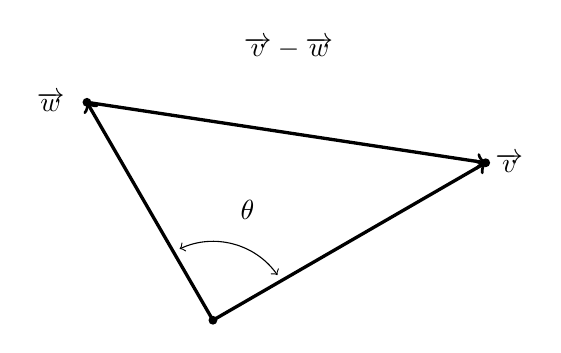
\begin{tikzpicture}[scale=0.8]

% Points
\fill (0,0) circle (2pt);
\fill (-2,3.46) circle (2pt);
\fill (4.33,2.5) circle (2pt);

% Angle arc
\draw[<->] (35:1.25) arc[start angle=35,end angle=115,radius=1.25];
\node at (0.55,1.75) {$\theta$};

% Vectors
\draw[->,line width=1.2pt] (0,0) -- (-2,3.46);
\draw[->,line width=1.2pt] (0,0) -- (4.33,2.5);
\draw[->,line width=1.2pt] (-2,3.46) -- (4.33,2.5);

% Labels
\node[right] at (4.33,2.5) {$\overrightarrow{v}$};
\node[left] at (-2.2,3.46) {$\overrightarrow{w}$};
\node[above] at (1.2,4.0) {$\overrightarrow{v}-\overrightarrow{w}$};

\end{tikzpicture}
\end{minipage}
\hfill
\begin{minipage}{0.47\textwidth}
\centering
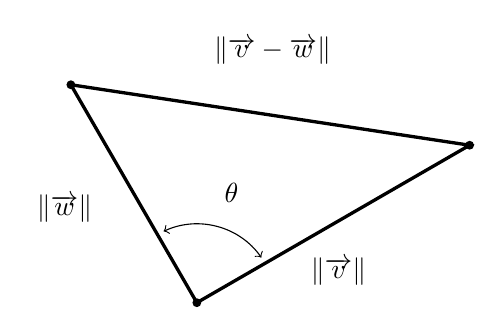
\begin{tikzpicture}[scale=0.8]

% Points
\fill (0,0) circle (2pt);
\fill (-2,3.46) circle (2pt);
\fill (4.33,2.5) circle (2pt);

% Angle arc
\draw[<->] (35:1.25) arc[start angle=35,end angle=115,radius=1.25];
\node at (0.55,1.75) {$\theta$};

% Triangle
\draw[line width=1.2pt]
    (0,0) -- (-2,3.46) -- (4.33,2.5) -- cycle;

% Labels
\node at (2.25,0.5) {$\|\overrightarrow{v}\|$};
\node at (-2.1,1.5) {$\|\overrightarrow{w}\|$};
\node at (1.2,4.0) {$\|\overrightarrow{v}-\overrightarrow{w}\|$};

\end{tikzpicture}
\end{minipage}

\end{center}

The Law of Cosines yields $\| \overrightarrow{v} - \overrightarrow{w} \|^2 = \|\overrightarrow{v}\|^2 + \|\overrightarrow{w}\|^2 - 2\|\overrightarrow{v}\| \|\overrightarrow{w}\| \cos(\theta)$.  From Example \ref{dotprodpropex}, we also have that $\|\overrightarrow{v} - \overrightarrow{w}\|^2 = \|\overrightarrow{v}\|^2  -2 (\overrightarrow{v} \cdot \overrightarrow{w}) + \|\overrightarrow{w}\|^2$.  

 

Equating these two expressions for $\| \overrightarrow{v} - \overrightarrow{w} \|^2$ gives $\|\overrightarrow{v}\|^2 + \|\overrightarrow{w}\|^2 - 2\|\overrightarrow{v}\| \|\overrightarrow{w}\| \cos(\theta)  =  \|\overrightarrow{v}\|^2  -2 (\overrightarrow{v} \cdot \overrightarrow{w}) + \|\overrightarrow{w}\|^2$ which reduces to $- 2\|\overrightarrow{v}\| \|\overrightarrow{w}\| \cos(\theta) =   -2 (\overrightarrow{v} \cdot \overrightarrow{w})$. Hence,  $\overrightarrow{v} \cdot \overrightarrow{w} = \|\overrightarrow{v}\| \|\overrightarrow{w}\| \cos(\theta)$, as required. 
 

An immediate consequence of Theorem \ref{dotproductgeo} is the following.

 

%% \colorbox{ResultColor}{\bbm

\begin{theorem} \label{anglebetweenvectorthm} Let $\overrightarrow{v}$ and $\overrightarrow{w}$ be nonzero vectors and let $\theta$ the angle between $\overrightarrow{v}$ and $\overrightarrow{w}$.  Then \index{vector ! angle between two} \index{angle ! between two vectors}

\[ \theta = \arccos\left( \frac{\overrightarrow{v} \cdot \overrightarrow{w}}{\| \overrightarrow{v} \| \|\overrightarrow{w} \|}\right) = \arccos(\hat{v} \cdot \hat{w}) \]

 

\end{theorem}

%% \ebm}

 

We obtain the formula in Theorem \ref{anglebetweenvectorthm} by solving the equation given in Theorem \ref{dotproductgeo} for $\theta$.  

 

Since $\overrightarrow{v}$ and $\overrightarrow{w}$ are nonzero, so are $\| \overrightarrow{v} \|$ and $\|\overrightarrow{w}\|$.  Hence, we may divide both sides of $\overrightarrow{v} \cdot \overrightarrow{w} = \| \overrightarrow{v} \| \|\overrightarrow{w} \| \cos(\theta)$ by $\| \overrightarrow{v} \| \|\overrightarrow{w} \|$.  Since $0 \leq \theta \leq \pi$ by definition, the values of $\theta$ exactly match the range of the arccosine function.  Hence,  \[ \cos(\theta) = \frac{\overrightarrow{v} \cdot \overrightarrow{w}}{\| \overrightarrow{v} \| \|\overrightarrow{w} \|} \, \Rightarrow \,  \theta = \arccos\left( \frac{\overrightarrow{v} \cdot \overrightarrow{w}}{\| \overrightarrow{v} \| \|\overrightarrow{w} \|}\right).\]

 

Using Theorem \ref{dotprodprops}, we can rewrite \[ \frac{\overrightarrow{v} \cdot \overrightarrow{w}}{\| \overrightarrow{v} \| \|\overrightarrow{w} \|} = \left(\frac{1}{\|\overrightarrow{v}\|} \overrightarrow{v}\right) \cdot \left(\frac{1}{\|\overrightarrow{w}\|} \overrightarrow{w}\right) = \hat{v} \cdot \hat{w},\]  giving us the alternative formula listed in Theorem \ref{anglebetweenvectorthm}:  $\theta = \arccos(\hat{v} \cdot \hat{w})$.    We are overdue for an example.

 

\begin{example} \label{anglebetweenvectorex}  Find the angle between the following pairs of vectors.  Graph each pair of vectors in standard position to check the reasonableness of your answer.
\begin{enumerate}

\item  \label{anglebetweenvectorexone} $\overrightarrow{v} = \left< 3, -3\sqrt{3} \right>$, and $\overrightarrow{w} = \left<-\sqrt{3}, 1 \right>$

\item  \label{anglebetweenvectorextwo} $\overrightarrow{v} = \left< 2, 2 \right>$, and $\overrightarrow{w} = \left<5, -5\right>$

\item \label{anglebetweenvectorexthree} $\overrightarrow{v} = \left< 3, -4 \right>$, and $\overrightarrow{w} = \left<2, 1\right>$

\end{enumerate}

\begin{explanation}
We use the formula $\theta = \arccos\left( \frac{\overrightarrow{v} \cdot \overrightarrow{w}}{\| \overrightarrow{v} \| \|\overrightarrow{w} \|}\right)$ from Theorem \ref{anglebetweenvectorthm} in each case below.

\begin{enumerate}

\item  We have $\overrightarrow{v} \cdot \overrightarrow{w} = \left< 3, -3\sqrt{3} \right> \cdot \left<-\sqrt{3}, 1 \right> = -3\sqrt{3} - 3\sqrt{3} = -6\sqrt{3}$.  Computing lengths of vectors, we find  $\| \overrightarrow{v} \| = \sqrt{3^2+(-3\sqrt{3})^2} = \sqrt{36} =6$ and $\| \overrightarrow{w}\| = \sqrt{(-\sqrt{3})^2+1^2} = \sqrt{4} =2$.  Hence,  we find $\theta = \arccos\left(\frac{-6\sqrt{3}}{12}\right) = \arccos\left(-\frac{\sqrt{3}}{2}\right) = \frac{5\pi}{6}$.  We check our answer geometrically by graphing this pair of vectors below.

\item  For $\overrightarrow{v} = \left< 2, 2 \right>$  and $\overrightarrow{w} = \left<5, -5\right>$, we find $\overrightarrow{v} \cdot \overrightarrow{w} = \left< 2, 2 \right> \cdot \left<5, -5\right> = 10-10 = 0$.  Hence, it doesn't matter what $\| \overrightarrow{v} \|$ and $\| \overrightarrow{w} \|$ are,  $\theta = \arccos\left( \frac{\overrightarrow{v} \cdot \overrightarrow{w}}{\| \overrightarrow{v} \| \|\overrightarrow{w} \|}\right) = \arccos(0) = \frac{\pi}{2}$.  We check our answer geometrically by graphing this pair of vectors below.

\begin{center}

\begin{minipage}{0.47\textwidth}
\centering

\begin{tikzpicture}[scale=0.5]

% Axes
\draw[->] (-3.2,0) -- (5.2,0);
\draw[->] (0,-5.4) -- (0,3.2);

\node[right] at (5,0) {\scriptsize $x$};
\node[above] at (0,3) {\scriptsize $y$};

% Origin
\fill (0,0) circle (2pt);

% Angle arc
\draw[<->]
  ({cos(157)},{sin(157)})
  arc[start angle=157,end angle=293,radius=1];

\node at (-2,-1) {$\theta=\dfrac{5\pi}{6}$};

% Vectors
\draw[->,line width=1.2pt] (0,0)--(3,-5.196);
\draw[->,line width=1.2pt] (0,0)--(-1.732,1);

% Labels
\node at (4,-4.5) {$\overrightarrow{v}$};
\node at (-2,1.5) {$\overrightarrow{w}$};

\end{tikzpicture}

\vspace{0.5em}

$\overrightarrow{v}$ and $\overrightarrow{w}$ from number~\ref{anglebetweenvectorexone}

\end{minipage}

\begin{minipage}{0.47\textwidth}
\centering

\begin{tikzpicture}[scale=0.5]

% Axes
\draw[->] (-3.2,0) -- (5.2,0);
\draw[->] (0,-5.4) -- (0,3.2);

\node[right] at (5,0) {\scriptsize $x$};
\node[above] at (0,3) {\scriptsize $y$};

% Origin
\fill (0,0) circle (2pt);

% Right-angle marker
\draw (0.3,0.3)--(0.6,0)--(0.3,-0.3);

\node at (2,-0.75) {$\theta=\dfrac{\pi}{2}$};

% Vectors
\draw[->,line width=1.2pt] (0,0)--(2,2);
\draw[->,line width=1.2pt] (0,0)--(5,-5);

% Labels
\node at (2.5,2) {$\overrightarrow{v}$};
\node at (5.5,-5) {$\overrightarrow{w}$};

\end{tikzpicture}

\vspace{0.5em}

$\overrightarrow{v}$ and $\overrightarrow{w}$ from number~\ref{anglebetweenvectorextwo}

\end{minipage}

\end{center}

\item  We find $\overrightarrow{v} \cdot \overrightarrow{w} = \left< 3, -4 \right> \cdot \left<2, 1\right> = 6 - 4 = 2$.  Computing lengths, we find $\| \overrightarrow{v} \| = \sqrt{3^2+(-4)^2} = \sqrt{25} = 5$ and $\overrightarrow{w} = \sqrt{2^2+1^2} = \sqrt{5}$, so $\theta = \arccos\left(\frac{2}{5\sqrt{5}}\right) = \arccos\left(\frac{2\sqrt{5}}{25} \right)$. 

 

Since $\frac{2\sqrt{5}}{25}$ isn't the cosine of one of the `common angles,' we leave our \textit{exact} answer in terms of the arccosine function. For the purposes of checking our answer, however, we  \textit{approximate} $\theta \approx 79.7^{\circ}$.



\begin{center}

\begin{tikzpicture}[scale=0.75]

% Axes
\draw[->] (-3.2,0) -- (5.2,0);
\draw[->] (0,-5.4) -- (0,3.2);

% Axis labels
\node[right] at (5,0) {\scriptsize $x$};
\node[above] at (0,3) {\scriptsize $y$};

% Origin
\fill (0,0) circle (2pt);

% Angle arc
\draw[<->]
    ({cos(-45)},{sin(-45)})
    arc[start angle=-45,end angle=19,radius=1];

\node[anchor=west] at (3.2,-1.8)
{$\theta=\arccos\!\left(\dfrac{2\sqrt5}{25}\right)\approx79.7^\circ$};

% Vectors
\draw[->,line width=1.2pt] (0,0)--(3,-4);
\draw[->,line width=1.2pt] (0,0)--(2,1);

% Labels
\node at (3.5,-4) {$\overrightarrow{v}$};
\node at (2.5,1) {$\overrightarrow{w}$};

\end{tikzpicture}

\vspace{0.5em}

$\overrightarrow{v}$ and $\overrightarrow{w}$ from number~\ref{anglebetweenvectorexthree}

\end{center}

\end{enumerate}
\end{explanation}
\end{example}

 

A few remarks about Example \ref{anglebetweenvectorex} are in order.  Note that for nonzero vectors $\overrightarrow{v}$ and $\overrightarrow{w}$, the lengths $\| \overrightarrow{v} \|$ and $\| \overrightarrow{w} \|$ are always positive. Since Theorem \ref{dotproductgeo} tells us that $\overrightarrow{v} \cdot \overrightarrow{w} =  \| \overrightarrow{v} \| \| \overrightarrow{w} \| \cos(\theta)$, we know the sign of $\overrightarrow{v} \cdot \overrightarrow{w}$ is the same as the sign of $\cos(\theta)$. 

 

Geometrically, if $\overrightarrow{v} \cdot \overrightarrow{w} < 0$, then $\cos(\theta) < 0$ so $\theta$ is an obtuse angle, demonstrated number \ref{anglebetweenvectorexone} above.  

 

If $\overrightarrow{v} \cdot \overrightarrow{w}  = 0$, then $\cos(\theta) = 0$ so $\theta = \frac{\pi}{2}$ as in number \ref{anglebetweenvectorextwo}. In this case, the vectors $\overrightarrow{v}$ and $\overrightarrow{w}$ are called \textbf{orthogonal}\index{vector ! orthogonal vectors}\index{orthogonal vectors}.  Geometrically, when orthogonal vectors are sketched with the same initial point, the lines containing the vectors are perpendicular. Hence, if $\overrightarrow{v}$ and $\overrightarrow{w}$ are orthogonal, we write $\overrightarrow{v} \perp \overrightarrow{w}$.    

 

Note there is no `zero product property' for the dot product.  As with the vectors in number \ref{anglebetweenvectorextwo} above, it is quite possible to have $\overrightarrow{v} \cdot \overrightarrow{w} = 0$ but neither $\overrightarrow{v}$ nor $\overrightarrow{w}$ be $\overrightarrow{0}$.

 
 
Finally, if $\overrightarrow{v} \cdot \overrightarrow{w} > 0$, then $\cos(\theta) > 0$ so $\theta$ is an acute angle, as in the case of number \ref{anglebetweenvectorexthree} above. 

 We summarize all of our observations in the schematic below.

\begin{center}

\begin{minipage}{0.31\textwidth}
\centering
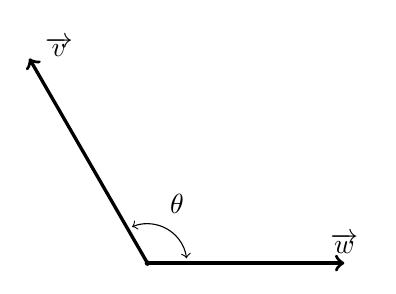
\begin{tikzpicture}[scale=0.5]

% Origin
\fill (0,0) circle (2pt);

% Angle arc
\draw[<->]
    ({cos(7)},{sin(7)})
    arc[start angle=7,end angle=113,radius=1];

\node at (0.75,1.5) {$\theta$};

% Vectors
\draw[->,line width=1.2pt] (0,0)--(5,0);
\draw[->,line width=1.2pt] (0,0)--({6*cos(120)},{6*sin(120)});

% Labels
\node at (5,0.5) {$\overrightarrow{w}$};
\node at (-2.25,5.5) {$\overrightarrow{v}$};

\end{tikzpicture}

$\overrightarrow{v}\cdot\overrightarrow{w}<0$

$\theta$ is obtuse

\end{minipage}
\hfill
\begin{minipage}{0.31\textwidth}
\centering
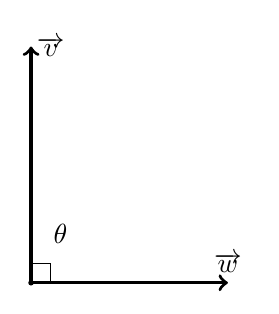
\begin{tikzpicture}[scale=0.5]

% Origin
\fill (0,0) circle (2pt);

% Right-angle marker
\draw (0,0.5)--(0.5,0.5)--(0.5,0);

\node at (0.75,1.25) {$\theta$};

% Vectors
\draw[->,line width=1.2pt] (0,0)--(5,0);
\draw[->,line width=1.2pt] (0,0)--({6*cos(90)},{6*sin(90)});

% Labels
\node at (5,0.5) {$\overrightarrow{w}$};
\node at (0.5,6) {$\overrightarrow{v}$};

\end{tikzpicture}

\vspace{0.5em}

$\overrightarrow{v}\cdot\overrightarrow{w}=0$

$\theta=\dfrac{\pi}{2}=90^\circ$

\end{minipage}
\hfill
\begin{minipage}{0.31\textwidth}
\centering
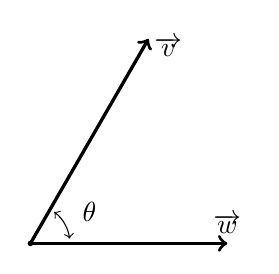
\begin{tikzpicture}[scale=0.5]

% Origin
\fill (0,0) circle (2pt);

% Angle arc
\draw[<->]
    ({cos(7)},{sin(7)})
    arc[start angle=7,end angle=53,radius=1];

\node at (1.5,0.8) {$\theta$};

% Vectors
\draw[->,line width=1.2pt] (0,0)--(5,0);
\draw[->,line width=1.2pt] (0,0)--({6*cos(60)},{6*sin(60)});

% Labels
\node at (5,0.5) {$\overrightarrow{w}$};
\node at (3.5,5) {$\overrightarrow{v}$};

\end{tikzpicture}

\vspace{0.5em}

$\overrightarrow{v}\cdot\overrightarrow{w}>0$

$\theta$ is acute

\end{minipage}

\end{center}

Of the three cases diagrammed above, the one which has the most mathematical significance moving forward is the orthogonal case.  Hence, we state the corresponding theorem below.

 

%% \colorbox{ResultColor}{\bbm
\begin{theorem} \label{dotprodorththm}   For nonzero vectors $\overrightarrow{v}$ and $\overrightarrow{w}$,  $\overrightarrow{v} \perp \overrightarrow{w}$ if and only if $\overrightarrow{v} \cdot \overrightarrow{w} = 0$. \index{vector ! dot product ! relation to orthogonality} \index{dot product ! relation to orthogonality}  

\end{theorem}
%% \ebm}

 

Basically,  Theorem \ref{dotprodorththm} tells us that  `the dot product detects orthogonality.'  This is a helpful interpretation to keep in mind as you continue your study of vectors in later courses.

 

We have already argued one direction of Theorem \ref{dotprodorththm}, namely if $\overrightarrow{v} \cdot \overrightarrow{w} = 0$ then $\overrightarrow{v} \perp \overrightarrow{w}$ in the comments following Example \ref{anglebetweenvectorex}. 

 

 To show the converse, we note if $\overrightarrow{v} \perp \overrightarrow{w}$, then the angle between $\overrightarrow{v}$ and $\overrightarrow{w}$, $\theta = \frac{\pi}{2}$.  From Theorem \ref{dotproductgeo}, we have that $\overrightarrow{v} \cdot \overrightarrow{w} = \| \overrightarrow{v} \| \| \overrightarrow{w} \| \cos \left( \frac{\pi}{2} \right) = \| \overrightarrow{v} \| \| \overrightarrow{w} \| \cdot (0) = 0$, as required.

 

We can use Theorem \ref{dotprodorththm} in the following example to provide a different proof about the relationship between the slopes of perpendicular lines.\footnote{See Exercise \ref{perpendicularlineproof} in Section \ref{AppLines}.}

\begin{example}\label{perpendicularlines2} Let $L_1$ be the line $y = m_1x + b_1$ and let $L_2$ be the line $y = m_2x + b_2$.  Prove that $L_1$ is perpendicular to $L_2$ if and only if $m_1 \cdot m_2 = -1$.

\begin{explanation}
Our strategy is to find two vectors: $\overrightarrow{v_1}$, which has the same direction as $L_1$,  and $\overrightarrow{v_2}$, which has the same direction as $L_2$ and show $\overrightarrow{v_1} \perp \overrightarrow{v_2}$ if and only if $ m_1  m_2 = -1$. 

 

 To that end, we substitute $x=0$ and $x=1$ into $y = m_1x + b_1$  to find two points which lie on $L_1$, namely $P(0,  b_1)$ and $Q(1, m_1 + b_1)$.  
 We let $\overrightarrow{v_1} = \overrightarrow{PQ} = \left<1-0,(m_1+b_1) - b_1\right>=\left<1,m_1\right>$.  Since  $\overrightarrow{v_1}$ is determined by two points on $L_1$, it may be viewed as lying on $L_1$, so $\overrightarrow{v_1}$  has the same direction as $L_1$. 
 
  
 
 Similarly, we get the vector  $\overrightarrow{v_2} = \left<1,m_2\right>$ which has the same direction as the line 
$L_2$.  Hence, $L_1$ and $L_2$ are perpendicular if and only if $\overrightarrow{v_1} \perp \overrightarrow{v_2}$. According to Theorem \ref{dotprodorththm}, $\overrightarrow{v_1} \perp \overrightarrow{v_2}$ if and only if $\overrightarrow{v_1} \cdot \overrightarrow{v_2} = 0$.  

 

Notice that $\overrightarrow{v_1} \cdot \overrightarrow{v_2} = \left<1,m_1\right> \cdot \left<1,m_2\right> = 1 + m_1m_2$.  Hence,  $\overrightarrow{v_1} \cdot \overrightarrow{v_2} = 0$ if and only if $1 + m_1m_2  =0$, which is true if and only if $ m_1  m_2 = -1$, as required. 

\end{explanation}
\end{example}

\subsection{Vector Projections}
\label{projections}

While Theorem \ref{dotprodorththm} certainly gives us some insight into what the dot product means geometrically, there is more to the story of the dot product.  Consider the two nonzero vectors $\overrightarrow{v}$ and $\overrightarrow{w}$ drawn with a common initial point $O$  below.  For the moment, assume that the angle between $\overrightarrow{v}$ and $\overrightarrow{w}$, $\theta$, is acute. 

\begin{center}
\begin{tikzpicture}[scale=0.8]

%%%%%%%%%%%%%%%%%%%%%%%%%%%%%%%%%%%%%%%%%%%%%%%%%%
% First picture
%%%%%%%%%%%%%%%%%%%%%%%%%%%%%%%%%%%%%%%%%%%%%%%%%%

\begin{scope}

% Origin
\fill (0,0) circle (2pt);
\node[below left] at (0,0) {$O$};

% Angle arc
\draw[<->]
({cos(40)},{sin(40)})
arc[start angle=40,end angle=80,radius=1];
\node at (0.75,1.5) {$\theta$};

% Vectors
\draw[->,line width=1.2pt]
(0,0)--({5*cos(30)},{5*sin(30)});

\draw[->,line width=1.2pt]
(0,0)--({6*cos(90)},{6*sin(90)});

% Labels
\node[right] at ({5*cos(30)},{5*sin(30)}) {$\vec w$};
\node[above] at ({6*cos(90)},{6*sin(90)}) {$\vec v$};

\end{scope}

%%%%%%%%%%%%%%%%%%%%%%%%%%%%%%%%%%%%%%%%%%%%%%%%%%
% Second picture
%%%%%%%%%%%%%%%%%%%%%%%%%%%%%%%%%%%%%%%%%%%%%%%%%%

\begin{scope}[xshift=8cm]

% Points
\fill (0,0) circle (2pt);
\fill ({3*cos(30)},{3*sin(30)}) circle (2pt);
\fill (0,6) circle (2pt);

\node[below left] at (0,0) {$O$};
\node[right] at ({3*cos(30)},{3*sin(30)}) {$R$};
\node[above] at (0,6) {$T$};

% Angle
\draw[<->]
({cos(40)},{sin(40)})
arc[start angle=40,end angle=80,radius=1];
\node at (0.75,1.5) {$\theta$};

% Vectors
\draw[->] (0,0)--({5*cos(30)},{5*sin(30)});
\draw[->] (0,0)--(0,6);
\draw[->,line width=1.2pt] (0,0)--({3*cos(30)},{3*sin(30)});

% Projection
\draw[dashed]
(0,6)--({3*cos(30)},{3*sin(30)});

% Right-angle mark
\draw
({3*cos(30)-0.2*sin(30)},{3*sin(30)+0.2*cos(30)})
--
({3*cos(30)-0.2*sin(30)-0.2*cos(30)},
 {3*sin(30)+0.2*cos(30)-0.2*sin(30)})
--
({3*cos(30)-0.4*cos(30)},
 {3*sin(30)-0.4*sin(30)});

% Labels
\node[right] at ({5*cos(30)},{5*sin(30)}) {$\vec w$};
\node[left] at (0,6) {$\vec v$};
\node[below] at ({1.75*cos(30)},{1.75*sin(30)})
{$\vec p=\overrightarrow{OR}$};

\end{scope}

%%%%%%%%%%%%%%%%%%%%%%%%%%%%%%%%%%%%%%%%%%%%%%%%%%
% Third picture
%%%%%%%%%%%%%%%%%%%%%%%%%%%%%%%%%%%%%%%%%%%%%%%%%%

\begin{scope}[xshift=16cm]

% Points
\fill (0,0) circle (2pt);
\fill ({3*cos(30)},{3*sin(30)}) circle (2pt);
\fill (0,6) circle (2pt);

\node[below left] at (0,0) {$O$};
\node[right] at ({3*cos(30)},{3*sin(30)}) {$R$};
\node[above] at (0,6) {$T$};

% Angle
\draw[<->]
({cos(40)},{sin(40)})
arc[start angle=40,end angle=80,radius=1];
\node at (0.75,1.5) {$\theta$};

% Triangle
\draw[line width=1.2pt]
(0,0)--({3*cos(30)},{3*sin(30)})
--(0,6)--cycle;

% Right-angle mark
\draw
({3*cos(30)-0.2*sin(30)},{3*sin(30)+0.2*cos(30)})
--
({3*cos(30)-0.2*sin(30)-0.2*cos(30)},
 {3*sin(30)+0.2*cos(30)-0.2*sin(30)})
--
({3*cos(30)-0.4*cos(30)},
 {3*sin(30)-0.4*sin(30)});

% Labels
\node[left] at (0,3) {$\|\vec v\|$};
\node[below] at ({1.5*cos(30)},{1.5*sin(30)})
{$\|\vec p\|$};

\end{scope}

\end{tikzpicture}
\end{center}

 We wish to develop a formula for the vector $\overrightarrow{p}$, indicated  below, which is called the \textbf{orthogonal projection of $\overrightarrow{v}$ onto $\overrightarrow{w}$}.\index{vector ! orthogonal projection}\index{projection ! orthogonal}\index{orthogonal projection}  The vector $\overrightarrow{p}$ is obtained geometrically as follows:  drop a perpendicular from the terminal point $T$ of $\overrightarrow{v}$ to the vector $\overrightarrow{w}$ and call the point of intersection $R$.  The vector $\overrightarrow{p}$ is then defined as $\overrightarrow{p} = \overrightarrow{OR}$.   

 

Like any vector, $\overrightarrow{p}$ is determined by its magnitude $\| \overrightarrow{p} \|$ and its direction $\hat{p}$ according to the formula $\overrightarrow{p} = \| \overrightarrow{p} \| \hat{p}$.  Since we want $\hat{p}$ to have the same direction as $\overrightarrow{w}$, we have $\hat{p} = \hat{w}$.  

 

To determine $\| \overrightarrow{p} \|$, we apply Definition \ref{righttrianglesinecosinetangent}  to the right triangle $\triangle ORT$.  We find $\cos(\theta) = \frac{\| \overrightarrow{p} \|}{\| \overrightarrow{v} \|}$, or, equivalently, $\| \overrightarrow{p} \| = \| \overrightarrow{v} \| \cos(\theta)$.  Using Theorems \ref{dotproductgeo} and \ref{dotprodprops}, we get:

 \[ \| \overrightarrow{p} \| = \| \overrightarrow{v} \| \cos(\theta) = \frac{ \| \overrightarrow{v} \| \| \overrightarrow{w} \| \cos(\theta)}{\| \overrightarrow{w} \|} = \frac{\overrightarrow{v} \cdot \overrightarrow{w}}{\|\overrightarrow{w}\|} =  \overrightarrow{v} \cdot \left(\frac{1}{\|\overrightarrow{w}\|} \overrightarrow{w}\right) = \overrightarrow{v} \cdot \hat{w}.\]

 

Hence, $\| \overrightarrow{p} \| = \overrightarrow{v} \cdot \hat{w}$, and since $\hat{p} = \hat{w}$, we have $\overrightarrow{p} = \| \overrightarrow{p} \| \hat{p} = (\overrightarrow{v} \cdot \hat{w}) \hat{w}$.

 

Now suppose that the angle $\theta$ between $\overrightarrow{v}$ and $\overrightarrow{w}$ is obtuse, and consider the diagram below. 

 

\begin{center}
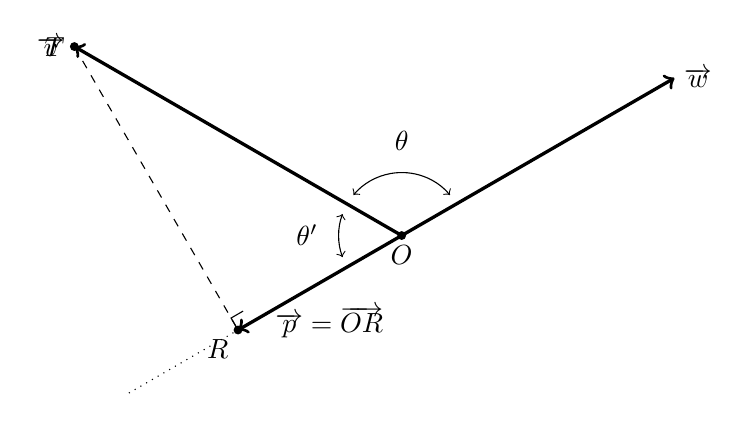
\begin{tikzpicture}[scale=0.8]

% Coordinates
\coordinate (O) at (0,0);
\coordinate (W) at ({5*cos(30)},{5*sin(30)});
\coordinate (T) at ({6*cos(150)},{6*sin(150)});
\coordinate (R) at ({3*cos(210)},{3*sin(210)});
\coordinate (L) at ({5*cos(210)},{5*sin(210)}); % extension of OR

% Points
\fill (O) circle (2pt);
\fill (R) circle (2pt);
\fill (T) circle (2pt);

% Labels
\node[below] at (O) {$O$};
\node[right] at (W) {$\overrightarrow{w}$};
\node[left] at (T) {$\overrightarrow{v}$};
\node[below left] at (R) {$R$};
\node[left] at (T) {$T$};
\node[below] at ({1.5*cos(220)},{1.5*sin(220)})
    {$\overrightarrow{p}=\overrightarrow{OR}$};

% Angle arcs
\draw[<->]
({cos(40)},{sin(40)})
arc[start angle=40,end angle=140,radius=1];

\node at (0,1.5) {$\theta$};

\draw[<->]
({cos(160)},{sin(160)})
arc[start angle=160,end angle=200,radius=1];

\node at (-1.5,0) {$\theta'$};

% Vectors
\draw[->,line width=1.2pt] (O)--(W);
\draw[->,line width=1.2pt] (O)--(T);
\draw[->,line width=1.2pt] (O)--(R);

% Dotted extension of p
\draw[dotted] (L)--(O);

% Dashed altitude
\draw[dashed] (T)--(R);

% Right-angle marker
\draw
({3*cos(210)},{3*sin(210)})
--
({3*cos(210)+0.22*cos(120)},{3*sin(210)+0.22*sin(120)})
--
({3*cos(210)+0.22*cos(120)+0.22*cos(30)},
 {3*sin(210)+0.22*sin(120)+0.22*sin(30)});

\end{tikzpicture}
\end{center}
 

In this case, we see that $\hat{p} = - \hat{w}$ and using the triangle $\triangle ORT$, we find $\| \overrightarrow{p} \| = \| \overrightarrow{v} \| \cos(\theta')$.   Since $\theta + \theta' = \pi$, it follows that $\cos(\theta') = -\cos(\theta)$, which means $\| \overrightarrow{p} \| = \| \overrightarrow{v} \| \cos(\theta') = - \| \overrightarrow{v} \| \cos(\theta)$.  

 

Rewriting this last equation in terms of $\overrightarrow{v}$ and $\overrightarrow{w}$ as before, we get $\|\overrightarrow{p} \| = -(\overrightarrow{v} \cdot \hat{w})$.  Putting this together with $\hat{p} = - \hat{w}$, we get $\overrightarrow{p} = \| \overrightarrow{p} \| \hat{p} = -(\overrightarrow{v} \cdot \hat{w}) (-\hat{w}) = (\overrightarrow{v} \cdot \hat{w}) \hat{w}$ in this case as well.

 


If the angle between $\overrightarrow{v}$ and $\overrightarrow{w}$ is $\frac{\pi}{2}$ then it is easy to show\footnote{In this case, the point $R$ coincides with the point $O$, so $\overrightarrow{p} =  \overrightarrow{OR} =  \overrightarrow{OO} = \overrightarrow{0}$.} that $\overrightarrow{p} = \overrightarrow{0}$. Since $\overrightarrow{v} \perp \overrightarrow{w}$ in this case, $\overrightarrow{v} \cdot \overrightarrow{w} = 0$.   It follows that $\overrightarrow{v} \cdot \hat{w} = 0$ and $\overrightarrow{p} = \overrightarrow{0} = 0 \hat{w} = (\overrightarrow{v} \cdot \hat{w}) \hat{w}$ in this case, too.  We have motivated the following.

 

%% \colorbox{ResultColor}{\bbm

\begin{definition} \label{vectorproj} Let $\overrightarrow{v}$ and $\overrightarrow{w}$ be nonzero vectors.  

 

The \textbf{orthogonal projection of $\overrightarrow{v}$ onto $\overrightarrow{w}$}, denoted $\text{proj}_{\overrightarrow{w}}(\overrightarrow{v})$ is given by $\text{proj}_{\overrightarrow{w}}(\overrightarrow{v}) = (\overrightarrow{v} \cdot \hat{w}) \hat{w}$.

 

\end{definition}
%% \ebm}

 

Definition \ref{vectorproj} gives us a good idea what the dot product does.  The scalar $\overrightarrow{v} \cdot \hat{w}$ is a measure of how much of the vector $\overrightarrow{v}$ is in the direction of the vector $\overrightarrow{w}$ and is thus called the \textbf{scalar projection}\index{scalar projection}\index{vector ! scalar projection} of $\overrightarrow{v}$ onto $\overrightarrow{w}$.  

 

While the formula given in Definition \ref{vectorproj} is theoretically appealing, because of the presence of the normalized unit vector $\hat{w}$, computing the projection using the formula $\text{proj}_{\overrightarrow{w}}(\overrightarrow{v}) = (\overrightarrow{v} \cdot \hat{w}) \hat{w}$ can be messy.  We present two other formulas that are often used in practice.

 

%% \colorbox{ResultColor}{\bbm

\begin{theorem} \label{altprojformulas} \textbf{Alternate Formulas for Vector Projections:}  If $\overrightarrow{v}$ and $\overrightarrow{w}$ are nonzero vectors then

\[\text{proj}_{\overrightarrow{w}}(\overrightarrow{v}) = (\overrightarrow{v} \cdot \hat{w}) \hat{w} = \left(\frac{\overrightarrow{v} \cdot \overrightarrow{w}}{\| \overrightarrow{w}\|^2}\right) \overrightarrow{w} = \left(\frac{\overrightarrow{v} \cdot \overrightarrow{w}}{\overrightarrow{w} \cdot \overrightarrow{w}}\right) \overrightarrow{w} \]

\end{theorem}
%% \ebm}

 

The proof of Theorem \ref{altprojformulas}, which we leave to the reader as an exercise, amounts to using the formula $\hat{w} = \left(\frac{1}{\| \overrightarrow{w} \|}\right) \overrightarrow{w}$ and properties of the dot product.  It is time for an example.

 

\begin{example} \label{projex}  Let $\overrightarrow{v} = \left<1,8\right>$ and $\overrightarrow{w} = \left<-1,2\right>$.  Find $\overrightarrow{p} = \text{proj}_{\overrightarrow{w}}(\overrightarrow{v})$.  Check your answer geometrically.

\begin{explanation}
We find $\overrightarrow{v} \cdot \overrightarrow{w} = \left<1,8\right> \cdot \left<-1,2\right> = (-1) + 16 = 15$ and $\overrightarrow{w} \cdot \overrightarrow{w} = \left<-1,2\right> \cdot \left<-1,2\right> = 1 + 4 = 5$.  Hence, \[\overrightarrow{p} = \frac{\overrightarrow{v} \cdot \overrightarrow{w}}{\overrightarrow{w} \cdot \overrightarrow{w}} \overrightarrow{w} = \frac{15}{5} \left<-1,2\right> = \left<-3,6\right> .\] We plot $\overrightarrow{v}$, $\overrightarrow{w}$ and $\overrightarrow{p}$ in standard position below on the left. We see $\overrightarrow{p}$ has the same direction as $\overrightarrow{w}$, but we need to do more to show  $\overrightarrow{p}$ in is indeed the \textit{orthogonal} projection of $\overrightarrow{v}$ onto $\overrightarrow{w}$. 

 

Consider the vector $\overrightarrow{q}$ whose initial point is the terminal point of $\overrightarrow{p}$ and whose terminal point is the terminal point of $\overrightarrow{v}$.  From the definition of vector arithmetic, $\overrightarrow{p} + \overrightarrow{q} = \overrightarrow{v}$, so that $\overrightarrow{q} = \overrightarrow{v} - \overrightarrow{p}$.  

 

Since $\overrightarrow{v} = \left<1,8\right>$ and $\overrightarrow{p} = \left<-3,6\right>$,  $\overrightarrow{q} = \left<1,8\right> - \left<-3,6\right> = \left<4,2\right>$.  To prove $\overrightarrow{q} \perp \overrightarrow{w}$, we compute the dot product:  $\overrightarrow{q} \cdot \overrightarrow{w} = \left<4,2\right> \cdot \left<-1,2\right> = (-4)+4  = 0$.  Hence, per  Theorem \ref{dotprodorththm}, we know $\overrightarrow{q} \perp \overrightarrow{w}$ which completes our check.\footnote{Note that, necessarily, $\overrightarrow{q} \perp \overrightarrow{p}$ as well!}

\begin{center}
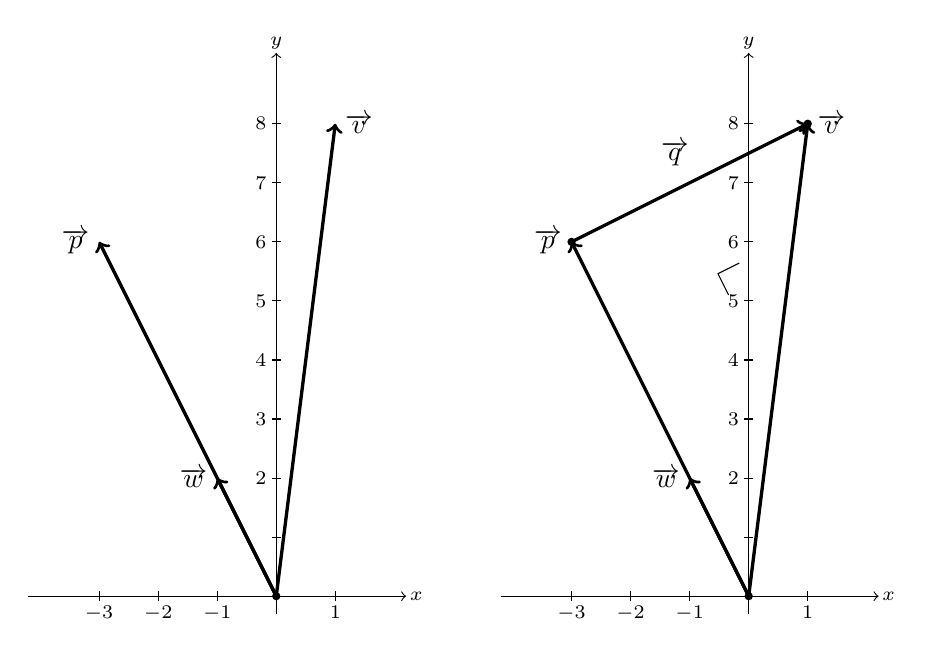
\begin{tikzpicture}[scale=0.75]

%%%%%%%%%%%%%%%%%%%%%%%%%%%%%%%%%%%%%%%%%%%%%%%%%%
% Left figure
%%%%%%%%%%%%%%%%%%%%%%%%%%%%%%%%%%%%%%%%%%%%%%%%%%

\begin{scope}

% Axes
\draw[->] (-4.2,0) -- (2.2,0);
\draw[->] (0,-0.3) -- (0,9.2);

% Tick marks
\foreach \x in {-3,-2,-1,1}
  \draw (\x,0.08)--(\x,-0.08);
\foreach \y in {1,...,8}
  \draw (0.08,\y)--(-0.08,\y);

% Tick labels
\foreach \x in {-3,-2,-1,1}
  \node[below] at (\x,0) {\scriptsize $\x$};

\foreach \y in {2,...,8}
  \node[left] at (0,\y) {\scriptsize $\y$};

% Axis labels
\node[right] at (2.1,0) {\scriptsize $x$};
\node[above] at (0,9.1) {\scriptsize $y$};

% Origin
\fill (0,0) circle (2pt);

% Vectors
\draw[->,line width=1.2pt] (0,0)--(1,8);
\draw[->,line width=1.2pt] (0,0)--(-1,2);
\draw[->,line width=1.2pt] (0,0)--(-3,6);

% Labels
\node[right] at (1,8) {$\overrightarrow{v}$};
\node[left] at (-1,2) {$\overrightarrow{w}$};
\node[left] at (-3,6) {$\overrightarrow{p}$};

\end{scope}

%%%%%%%%%%%%%%%%%%%%%%%%%%%%%%%%%%%%%%%%%%%%%%%%%%
% Right figure
%%%%%%%%%%%%%%%%%%%%%%%%%%%%%%%%%%%%%%%%%%%%%%%%%%

\begin{scope}[xshift=8cm]

% Axes
\draw[->] (-4.2,0) -- (2.2,0);
\draw[->] (0,-0.3) -- (0,9.2);

% Tick marks
\foreach \x in {-3,-2,-1,1}
  \draw (\x,0.08)--(\x,-0.08);
\foreach \y in {1,...,8}
  \draw (0.08,\y)--(-0.08,\y);

% Tick labels
\foreach \x in {-3,-2,-1,1}
  \node[below] at (\x,0) {\scriptsize $\x$};

\foreach \y in {2,...,8}
  \node[left] at (0,\y) {\scriptsize $\y$};

% Axis labels
\node[right] at (2.1,0) {\scriptsize $x$};
\node[above] at (0,9.1) {\scriptsize $y$};

% Points
\fill (0,0) circle (2pt);
\fill (-3,6) circle (2pt);
\fill (1,8) circle (2pt);

% Vectors
\draw[->,line width=1.2pt] (0,0)--(1,8);
\draw[->,line width=1.2pt] (0,0)--(-1,2);
\draw[->,line width=1.2pt] (0,0)--(-3,6);
\draw[->,line width=1.2pt] (-3,6)--(1,8);

% Right-angle marker
\draw
(-0.16,5.64)--(-0.52,5.46)--(-0.34,5.10);

% Labels
\node[right] at (1,8) {$\overrightarrow{v}$};
\node[left] at (-1,2) {$\overrightarrow{w}$};
\node[left] at (-3,6) {$\overrightarrow{p}$};
\node at (-1.25,7.5) {$\overrightarrow{q}$};

\end{scope}

\end{tikzpicture}
\end{center}
\end{explanation}
\end{example}
 

In Example \ref{projex} above, writing $\overrightarrow{v} = \overrightarrow{p} + \overrightarrow{q}$ is an example of what is called a \index{decomposition ! vector}\index{vector decomposition}\textbf{vector decomposition} of $\overrightarrow{v}$.  We generalize this result in the following theorem.
 
 

%% \colorbox{ResultColor}{\bbm

\begin{theorem} \label{generalizeddecompthm}  \textbf{Generalized Decomposition Theorem:} \index{vector ! Decomposition Theorem ! Generalized} Let $\overrightarrow{v}$ and $\overrightarrow{w}$ be nonzero vectors.  There are unique vectors $\overrightarrow{p}$ and $\overrightarrow{q}$  such that $\overrightarrow{v} = \overrightarrow{p} + \overrightarrow{q}$ where $\overrightarrow{p} = k \overrightarrow{w}$ for some scalar $k$, and $\overrightarrow{q} \cdot \overrightarrow{w} = 0$.

\end{theorem}


%% \ebm}

 

If the vectors $\overrightarrow{p}$ and $\overrightarrow{q}$ in Theorem \ref{generalizeddecompthm} are  nonzero, then we can say $\overrightarrow{p}$ is `parallel'\footnote{See Exercise \ref{parallelvectorexercise} in Section \ref{Vectors}.} to $\overrightarrow{w}$ and $\overrightarrow{q}$ is  `orthogonal' to $\overrightarrow{w}$. In this case, the vector $\overrightarrow{p}$ is sometimes called the `vector component of $\overrightarrow{v}$ \textit{parallel} to $\overrightarrow{w}$' and $\overrightarrow{q}$ is called the `vector component of $\overrightarrow{v}$ \textit{orthogonal} to $\overrightarrow{w}$.' 

 

To prove Theorem \ref{generalizeddecompthm}, we take  $\overrightarrow{p} = \text{proj}_{\overrightarrow{w}}(\overrightarrow{v})$ and $\overrightarrow{q} = \overrightarrow{v} - \overrightarrow{p}$.  Then  $\overrightarrow{p}$ is, by definition, a scalar multiple of $\overrightarrow{w}$.  Next, we compute $\overrightarrow{q} \cdot \overrightarrow{w}$.

\[ \begin{array}{rcll}

\overrightarrow{q} \cdot \overrightarrow{w} & = & (\overrightarrow{v} - \overrightarrow{p}) \cdot \overrightarrow{w}& \text{Definition of $\overrightarrow{q}$.} \\ 
& = & \overrightarrow{v} \cdot \overrightarrow{w} - \overrightarrow{p} \cdot \overrightarrow{w} & \text{Properties of Dot Product} \\  
& = & \overrightarrow{v} \cdot \overrightarrow{w} - \left(\frac{\overrightarrow{v} \cdot \overrightarrow{w}}{\overrightarrow{w} \cdot \overrightarrow{w}} \overrightarrow{w}\right) \cdot \overrightarrow{w} & \text{Since $\overrightarrow{p} = \text{proj}_{\overrightarrow{w}}(\overrightarrow{v})$.} \\  
& = & \overrightarrow{v} \cdot \overrightarrow{w} - \left(\frac{\overrightarrow{v} \cdot \overrightarrow{w}}{\overrightarrow{w} \cdot \overrightarrow{w}}\right) (\overrightarrow{w} \cdot \overrightarrow{w}) & \text{Properties of Dot Product.} \\  
& = & \overrightarrow{v} \cdot \overrightarrow{w} - \overrightarrow{v}\cdot \overrightarrow{w} & \\ 
& = & 0. & \end{array} \]
											
Hence, $\overrightarrow{q} \cdot \overrightarrow{w} = 0$, as required.  At this point, we have shown that the vectors $\overrightarrow{p}$ and $\overrightarrow{q}$ guaranteed by Theorem \ref{generalizeddecompthm} \textit{exist}.  Now we need to show that they are \textit{unique} - that is, there is only \textit{one} such way to decompose $\overrightarrow{v}$ in the manner described in  Theorem \ref{generalizeddecompthm}.

Suppose $\overrightarrow{v} = \overrightarrow{p} + \overrightarrow{q} = \overrightarrow{p} \,' + \overrightarrow{q} \,'$ where the vectors $\overrightarrow{p} \,'$ and $\overrightarrow{q} \,'$ satisfy the same properties described in  Theorem \ref{generalizeddecompthm} as $\overrightarrow{p}$ and $\overrightarrow{q}$.  Then $\overrightarrow{p} - \overrightarrow{p} \,' = \overrightarrow{q} \,' - \overrightarrow{q}$, so $\overrightarrow{w} \cdot (\overrightarrow{p} - \overrightarrow{p} \,') = \overrightarrow{w} \cdot (\overrightarrow{q} \,' - \overrightarrow{q}) = \overrightarrow{w} \cdot \overrightarrow{q} \,' - \overrightarrow{w} \cdot \overrightarrow{q} = 0 - 0 = 0$.  The long and short of this computation is that $\overrightarrow{w} \cdot (\overrightarrow{p} - \overrightarrow{p} \,') = 0$. 

 

Now there are scalars $k$ and $k \,'$ so that $\overrightarrow{p} = k \overrightarrow{w}$ and $\overrightarrow{p} \,' = k\,'\overrightarrow{w}$.   This means  $\overrightarrow{w} \cdot (\overrightarrow{p} - \overrightarrow{p} \,') = \overrightarrow{w} \cdot ( k \overrightarrow{w} - k \,' \overrightarrow{w}) = \overrightarrow{w} \cdot ([k - k \,'] \overrightarrow{w}) = (k - k \,') (\overrightarrow{w} \cdot \overrightarrow{w}) = (k - k \,') \| \overrightarrow{w} \|^2$.  

 

Since $\overrightarrow{w} \neq \overrightarrow{0}$, $\| \overrightarrow{w} \|^2 \neq 0$, which means the only way $\overrightarrow{w} \cdot (\overrightarrow{p} - \overrightarrow{p} \,') = (k - k \,') \| \overrightarrow{w} \|^2  = 0$ is for $k - k \,' = 0$, or $k = k \,'$.  This means $\overrightarrow{p} = k \overrightarrow{w} = k \,' \overrightarrow{w} = \overrightarrow{p} \,'$.  Since $\overrightarrow{q} \,' - \overrightarrow{q} = \overrightarrow{p} - \overrightarrow{p} \,' = \overrightarrow{p} - \overrightarrow{p} = \overrightarrow{0}$, it must be that $\overrightarrow{q} \,' = \overrightarrow{q}$ as well.  

 

Hence, we have shown there is only one way to write $\overrightarrow{v}$ as a sum of vectors as described in Theorem  \ref{generalizeddecompthm}, so the decomposition listed there is unique.

 


We close this section with an application of the dot product. In Physics, if a constant force $F$ is exerted over a distance $d$, the \index{work} \textbf{work} $W$ done by the force is given by $W = Fd$. Here, the assumption is that the force is being applied in the direction of the motion.  If the force applied is not in the direction of the motion, we can use the dot product to find the work done.  

 

Consider the scenario sketched below in which  the constant force $\overrightarrow{F}$ is applied to move an object from the point $P$ to the point $Q$.  Here the force is being applied at an angle $\theta$ as opposed to being applied directly in the direction of the motion.

\begin{center}
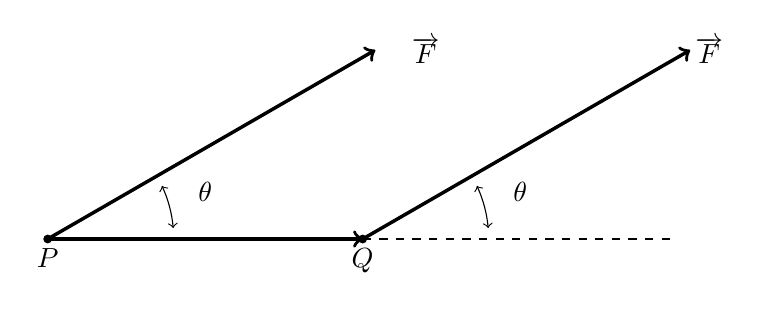
\begin{tikzpicture}[scale=0.8]

% Points
\fill (-5,0) circle (2pt);
\fill (0,0) circle (2pt);

% Labels for points
\node[below] at (-5,0) {$P$};
\node[below] at (0,0) {$Q$};

% Ground line
\draw[dashed] (0,0)--(5,0);

% Angle arcs
\draw[<->]
({2*cos(5)-5},{2*sin(5)})
arc[start angle=5,end angle=25,radius=2];

\draw[<->]
({2*cos(5)},{2*sin(5)})
arc[start angle=5,end angle=25,radius=2];

% Angle labels
\node at (-2.5,0.75) {$\theta$};
\node at (2.5,0.75) {$\theta$};

% Force vectors
\draw[->,line width=1.25pt] (-5,0)--(0.2,3);
\draw[->,line width=1.25pt] (0,0)--(5.2,3);
\draw[->,line width=1.25pt] (-5,0)--(0,0);

% Force labels
\node at (5.5,3) {$\overrightarrow{F}$};
\node at (1,3) {$\overrightarrow{F}$};

\end{tikzpicture}
\end{center}

To find the work $W$ done in this scenario, we need to find how much of the force $\overrightarrow{F}$ is  in the \text{direction} of the motion $\overrightarrow{PQ}$.  This is precisely what the dot product $\overrightarrow{F} \cdot \widehat{PQ}$ represents.  

 

Since the distance the object travels is $\| \overrightarrow{PQ} \|$, we get $W = (\overrightarrow{F} \cdot \widehat{PQ}) \| \overrightarrow{PQ} \|$.  Since $\overrightarrow{PQ} = \|\overrightarrow{PQ}\| \widehat{PQ}$, we can simplify this formula as follows:   $W = (\overrightarrow{F} \cdot \widehat{PQ}) \| \overrightarrow{PQ} \| = \overrightarrow{F} \cdot ( \| \overrightarrow{PQ} \|\widehat{PQ} ) = \overrightarrow{F} \cdot \overrightarrow{PQ}$.

 

Using Theorem \ref{dotproductgeo}, we can rewrite  $W = \overrightarrow{F} \cdot \overrightarrow{PQ} =  \| \overrightarrow{F} \| \| \overrightarrow{PQ} \| \cos(\theta)$, where $\theta$ is the angle between the applied force $\overrightarrow{F}$ and the trajectory of the motion $\overrightarrow{PQ}$.  We have proved the following.

 
%% \colorbox{ResultColor}{\bbm

\begin{theorem} \label{workthm}\index{dot product ! work}\index{vector ! dot product ! work} \textbf{Work as a Dot Product:}  Suppose a constant force $\overrightarrow{F}$ is applied along the vector $\overrightarrow{PQ}$.  The work $W$ done by $\overrightarrow{F}$ is given by

\[ W = \overrightarrow{F} \cdot \overrightarrow{PQ}  = \| \overrightarrow{F} \| \| \overrightarrow{PQ} \| \cos(\theta),\]

where $\theta$ is the angle between $\overrightarrow{F}$ and $\overrightarrow{PQ}$.

\end{theorem}

%% \ebm}

 

We test out our formula for work in the following example.

 

\begin{example}  \label{vectorworkex} Taylor exerts a force of $10$ pounds to pull her wagon a distance of $50$ feet over level ground.  If the handle of the wagon makes a $30^{\circ}$ angle with the horizontal, how much work did Taylor do pulling the wagon? Assume  the force of $10$ pounds is exerted at a $30^{\circ}$ angle for the duration of the $50$ feet.

\begin{center}
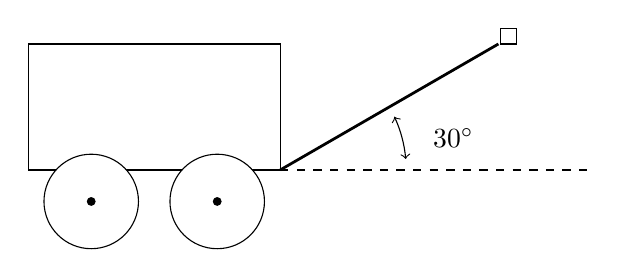
\begin{tikzpicture}[scale=0.8]

% Dashed horizontal reference line
\draw[dashed] (0,0) -- (5,0);

% Angle arc
\draw[<->]
  ({2*cos(5)},{2*sin(5)})
  arc[start angle=5,end angle=25,radius=2];

\node at (2.75,0.5) {$30^\circ$};

% Inclined segment
\draw[line width=1.0pt] (0,0) -- ({4*cos(30)},{4*sin(30)});

% Small square at end of inclined segment
\draw (3.5,2) rectangle (3.75,2.25);

% Large rectangle
\draw (-4,0) rectangle (0,2);

% Wheels (white-filled circles)
\filldraw[fill=white] (-3,-0.5) circle (0.75);
\filldraw[fill=white] (-1,-0.5) circle (0.75);

% Wheel centers
\fill (-3,-0.5) circle (2pt);
\fill (-1,-0.5) circle (2pt);

\end{tikzpicture}
\end{center}

\begin{explanation}
There are (at least) two ways to attack this problem.  One way is to find the vectors $\overrightarrow{F}$ and $\overrightarrow{PQ}$ mentioned in Theorem \ref{workthm} and compute $W = \overrightarrow{F} \cdot \overrightarrow{PQ}$.  

 

To do this, we assume the origin is at the point where the handle of the wagon meets the wagon and the positive $x$-axis lies along the dashed line in the figure above. 
 

 To find the force vector $\overrightarrow{F}$, we note the force in this situation is a constant 10 pounds, so  $\|\overrightarrow{F}\| = 10$.   Moreover, the force  is being applied at a constant angle of $\theta = 30^{\circ}$ with respect to the positive $x$-axis.    Definition \ref{polarformvector} gives us $\overrightarrow{F} = \| \overrightarrow{F} \| \left< \cos(\theta), \sin(\theta) \right> = 10 \left<\cos(30^{\circ}, \sin(30^{\circ})\right> = \left<5\sqrt{3}, 5\right>$.

 

  Since the wagon is being pulled along 50 feet in the positive $x$-direction, we find the displacement vector is $\overrightarrow{PQ} = 50 \hat{\text{i}} = 50\left<1,0\right> = \left<50,0\right>$.  
  
 
  
Per Theorem \ref{workthm},  $W = \overrightarrow{F} \cdot \overrightarrow{PQ} = \left<5\sqrt{3}, 5\right> \cdot \left<50,0\right> = 250\sqrt{3}$.  Since  force is measured in pounds and distance is measured in feet, we get $W = 250\sqrt{3}$ foot-pounds.  
  
 
  
 Alternatively, we can use the formula $W =  \| \overrightarrow{F} \| \| \overrightarrow{PQ} \| \cos(\theta)$.  With $\| \overrightarrow{F} \| = 10$ pounds, $\| \overrightarrow{PQ} \| = 50$ feet and $\theta = 30^{\circ}$, we get $W = (10 \, \text{pounds})(50 \, \text{feet}) \cos\left(30^{\circ}\right) = 250 \sqrt{3}$ foot-pounds of work. 
\end{explanation}
\end{example}


%% SKIPPED %% \documentclass{ximera}

\begin{document}
	\author{Stitz-Zeager}
	\xmtitle{Exercises for The Dot Product}{}

\mfpicnumber{1} \opengraphsfile{ExercisesforTheDotProduct} % mfpic settings added 

\begin{question}
In Exercises \ref{dotprodbasicfirst} - \ref{dotprodbasiclast}, use the pair of vectors $\vec{v}$ and $\vec{w}$ to find the following quantities.

\begin{itemize}

\item $\vec{v} \cdot \vec{w}$
\item The angle $\theta$ (in degrees) between $\vec{v}$ and $\vec{w}$ 
\item $\text{proj}_{\vec{w}}(\vec{v})$
\item $\vec{q} = \vec{v} - \text{proj}_{\vec{w}}(\vec{v})$ (Show that $\vec{q} \cdot \vec{w} = 0$.)

\end{itemize}

\begin{problem} \label{dotprodbasicfirst}
$\vec{v} = \left\langle -2, -7 \right\rangle$ and $\vec{w} = \left\langle 5, -9 \right\rangle$ 
\end{problem}

\begin{problem}
 $\vec{v} = \left\langle -6, -5 \right\rangle$ and $\vec{w} = \left\langle 10, -12 \right\rangle$
 \end{problem}

\begin{problem}
$\vec{v} = \left\langle 1, \sqrt{3} \right\rangle$ and $\vec{w} = \left\langle 1, -\sqrt{3} \right\rangle$
\end{problem}

\begin{problem}
$\vec{v} = \left\langle  3, 4 \right\rangle$ and $\vec{w} = \left\langle -6, -8 \right\rangle$
\end{problem}

\begin{problem}
$\vec{v} = \left\langle -2,1 \right\rangle$ and $\vec{w} = \left\langle 3,6 \right\rangle$
\end{problem}

\begin{problem}
$\vec{v} = \left\langle -3\sqrt{3}, 3\right\rangle$ and $\vec{w} = \left\langle -\sqrt{3}, -1 \right\rangle$
\end{problem}

\begin{problem}
$\vec{v} = \left\langle 1, 17 \right\rangle$ and $\vec{w} = \left\langle -1, 0 \right\rangle$
\end{problem}

\begin{problem}
$\vec{v} = \left\langle 3, 4 \right\rangle$ and $\vec{w} = \left\langle 5, 12 \right\rangle$
\end{problem}

\begin{problem}
$\vec{v} = \left\langle -4, -2 \right\rangle$ and $\vec{w} = \left\langle 1, -5 \right\rangle$
\end{problem}

\begin{problem}
$\vec{v} = \left\langle -5, 6 \right\rangle$ and $\vec{w} = \left\langle 4, -7 \right\rangle$
\end{problem}

\begin{problem}
$\vec{v} = \left\langle -8, 3 \right\rangle$ and $\vec{w} = \left\langle 2, 6 \right\rangle$
\end{problem}

\begin{problem}
$\vec{v} = \left\langle 34, -91 \right\rangle$ and $\vec{w} = \left\langle 0, 1 \right\rangle$
\end{problem}

\begin{problem}
$\vec{v} =3 \bm\hat{\text{i}}-  \bm\hat{\text{j}}$ and $\vec{w} = 4 \bm\hat{\text{j}}$
\end{problem}

\begin{problem}
$\vec{v} = -24 \bm\hat{\text{i}}+ 7 \bm\hat{\text{j}}$ and $\vec{w} = 2 \bm\hat{\text{i}}$
\end{problem}

\begin{problem}
$\vec{v} =\frac{3}{2}  \bm\hat{\text{i}}+ \frac{3}{2}  \bm\hat{\text{j}}$ and $\vec{w} =  \bm\hat{\text{i}}-  \bm\hat{\text{j}}$
\end{problem}

\begin{problem}
$\vec{v} = 5 \bm\hat{\text{i}}+12 \bm\hat{\text{j}}$ and $\vec{w} = -3 \bm\hat{\text{i}}+ 4 \bm\hat{\text{j}}$
\end{problem}

\begin{problem}
$\vec{v} = \left\langle \frac{1}{2}, \frac{\sqrt{3}}{2} \right\rangle$ and $\vec{w} = \left\langle -\frac{\sqrt{2}}{2}, \frac{\sqrt{2}}{2} \right\rangle$
\end{problem}

\begin{problem}
$\vec{v} = \left\langle \frac{\sqrt{2}}{2}, \frac{\sqrt{2}}{2} \right\rangle$ and $\vec{w} = \left\langle \frac{1}{2}, -\frac{\sqrt{3}}{2} \right\rangle$
\end{problem}

\begin{problem}
$\vec{v} = \left\langle \frac{\sqrt{3}}{2}, \frac{1}{2} \right\rangle$ and $\vec{w} = \left\langle -\frac{\sqrt{2}}{2}, -\frac{\sqrt{2}}{2} \right\rangle$
\end{problem}

\begin{problem} \label{dotprodbasiclast}
$\vec{v} = \left\langle \frac{1}{2}, -\frac{\sqrt{3}}{2} \right\rangle$ and $\vec{w} = \left\langle \frac{\sqrt{2}}{2}, -\frac{\sqrt{2}}{2} \right\rangle$
\end{problem}


\end{question}

\begin{problem}
A force of $1500$ pounds is required to tow a trailer.  Find the work done towing the trailer along a flat stretch of road $300$ feet.  Assume the force is applied in the direction of the motion.
\end{problem}

\begin{problem}
Find the work done lifting a $10$ pound book $3$ feet straight up into the air.  Assume the force of gravity is acting straight downwards.
\end{problem}

\begin{problem}
Suppose Taylor fills her wagon with rocks and must exert a force of 13 pounds to pull her wagon across the yard.  If she maintains a $15^{\circ}$ angle between the handle of the wagon and the horizontal, compute how much work Taylor does pulling her wagon 25 feet.  Round your answer to two decimal places.
\end{problem}

\begin{problem}
In Exercise \ref{kegpull} in Section \ref{Vectors}, two drunken college students have filled an empty beer keg with rocks which they drag down the street by pulling on two attached ropes.  The stronger of the two students pulls with a force of 100 pounds on a rope which makes a $13^{\circ}$ angle with the direction of motion.  (In this case, the keg was being pulled due east and the student's heading was N$77^{\circ}$E.)  Find the work done by this student if the keg is dragged 42 feet.
\end{problem}

\begin{problem}
Find the work done pushing a 200 pound barrel 10 feet up a $12.5^{\circ}$ incline. Ignore all forces acting on the barrel except gravity, which acts downwards.  Round your answer to two decimal places.

\textbf{HINT:}  Since you are working to overcome gravity only, the force being applied acts directly upwards. This means that the angle between the applied force in this case and the motion of the object is \textit{not} the $12.5^{\circ}$ of the incline!
\end{problem}

\begin{problem}
Prove the distributive property of the dot product in Theorem \ref{dotprodprops}.
\end{problem}

\begin{problem}
Finish the proof of the scalar property of the dot product in Theorem \ref{dotprodprops}.
\end{problem}

\begin{problem}
Show Theorem \ref{generalizeddecompthm} reduces to Theorem \ref{ijdecomp} in the case $\vec{w} =  \bm\hat{\text{i}}$.
\end{problem}

\begin{problem}
Use the identity in Example \ref{dotprodpropex} to prove the \href{http://en.wikipedia.org/wiki/Parallelogram_law}{\underline{\textbf{Parallelogram Law}}}

\[ \|\vec{v}\|^2 + \|\vec{w}\|^2 = \frac{1}{2}\left[ \| \vec{v} + \vec{w}\|^2 + \|\vec{v} - \vec{w}\|^2\right] \]
\end{problem}

\begin{problem} \label{triangleineqforvectorsexercise} 
We know that $|x + y| \leq |x| + |y|$ for all real numbers $x$ and $y$ by the Triangle Inequality established in Exercise \ref{triangleinequalityreals} in Section \ref{AbsoluteValueFunctions}.  We can now establish a Triangle Inequality for vectors.  In this exercise, we prove that $\| \vec{u} + \vec{v} \| \leq \| \vec{u} \| + \| \vec{v} \|$ for all pairs of vectors $\vec{u}$ and $\vec{v}$. \index{vector ! triangle inequality}

\begin{enumerate}

\item (Step 1) Show that $\| \vec{u} + \vec{v} \|^{2} = \| \vec{u} \|^{2} + 2\vec{u} \cdot \vec{v} + \| \vec{v} \|^{2}$.

\item (Step 2) Show that $|\vec{u} \cdot \vec{v}| \leq \| \vec{u} \| \| \vec{v} \|$.  This is the celebrated Cauchy-Schwarz Inequality.\footnote{It is also known by other names.  Check out this \href{http://en.wikipedia.org/wiki/Cauchy-Schwarz_inequality}{\underline{site}} for details.} 

\smallskip

HINT:  Start with $|\vec{u} \cdot \vec{v}| = |\; \| \vec{u} \| \| \vec{v} \|\cos(\theta) \;|$ and use the fact that $|\cos(\theta)| \leq 1$ for all $\theta$.

\item (Step 3) Show: \[\| \vec{u} + \vec{v} \|^{2} = \| \vec{u} \|^{2} + 2\vec{u} \cdot \vec{v} + \| \vec{v} \|^{2} \leq \| \vec{u} \|^{2} + 2|\vec{u} \cdot \vec{v}| + \| \vec{v} \|^{2} \leq \| \vec{u} \|^{2} + 2\| \vec{u} \| \| \vec{v} \| + \| \vec{v} \|^{2} = (\| \vec{u} \| + \| \vec{v} \|)^{2}.\]

\item (Step 4) Use Step 3 to show that $\| \vec{u} + \vec{v} \| \leq \| \vec{u} \| + \| \vec{v} \|$ for all pairs of vectors $\vec{u}$ and $\vec{v}$.

\end{enumerate}

\end{problem}

\end{document}

\closegraphsfile

\end{document}
